\section{Further Mechanics (for Paper 3)}
\subsection{Motion of a projectile}
\begin{point}
Model the motion of a projectile as a particle
moving with constant acceleration and
understand any limitations of the model
\end{point}
A \define{projectile} is any object that, once it has been thrown, propelled or
dropped, continues to move under its own inertia and the force of gravity. From
Advanced Level Mechanics, we know that
\begin{itemize}
	\item $s = ut + \frac{1}{2}at^2$
	\item $v = u + at$
	\item $v^2 = u^2 + 2as$
	\item $s = \frac{1}{2}(u+v)t$
	\item $s = vt - \frac{1}{2}at^2$
\end{itemize}

To predict the motion of projectiles, we make certain assumptions. We assume
the absence of air resistance, no rotational forces (spin) affect the 
projectile since we consider it to be a \emph{particle} (no volume) and that
force due to gravity is constant. The path travelled by a projectile is known
as a \define{parabolic trajectory}.
\begin{point}
Use horizontal and vertical equations of motion
to solve problems on the motion of projectiles,
including finding the magnitude and direction
of the velocity at a given time or position, the
range on a horizontal plane and the greatest
height reached
\end{point}
Consider a particle thrown with initial speed $u$, at an angle $\theta$
above the horizontal direction. Thus the horizontal and vertical components
of the velocity is $u \cos \theta$ and $u \sin \theta$, respectively. Thus,
from $v = u + at$
$$ \boxed{v_x = u\sin\theta} $$
since there is no acceleration in the $x$-direction. The acceleration in the
$y$-direction is that of gravity, in the downward direction, $-g$. Hence
$$ \boxed{v_y = u \cos\theta - gt} $$

At the peak of the particle's motion, 
\begin{align*}
	v_y &= 0 \\
	\implies u \sin \theta &= gt \\
	\implies \Aboxed{t &= \frac{u \sin\theta}{g}}
\end{align*}

Since air resistance is ignored, the time for the particle to reach its peak
is the same for the particle to drop back down to its original position, thus
the total time for the motion is
$$ \boxed{t = \frac{2u \sin \theta}{g}} $$

Now, taking $x$ as horizontal displacement and $y$ as vertical displacement,
using $s = ut + \frac{1}{2}at^2$, we have
\begin{align*}
	x &= u \cos\theta \frac{2u\sin\theta}{g} \\
	  &= \frac{2u^2\sin\theta\cos\theta}{g}
\end{align*}
recalling that $2\sin\theta\cos\theta \equiv 2\sin 2\theta$, we have
$$\boxed{x = \frac{u^2\sin 2\theta}{g}}$$

The above is called the \define{range} of the projectile's motion. This
value is at a maximum when $\theta = 45^{\circ}$, i.e., when $\sin 2\theta = 1$.

The maximum height of the projectile is derived as follows
\begin{align*}
	y &= \left(u\sin\theta\right)\left(\frac{u\sin\theta}{g}\right) \\
	\Aboxed{&= \frac{u^2 \sin^2\theta}{g}}
\end{align*}

When an object begins its motion from a certain height above the horizontal. We
can use $v^2 = u^2 + 2as$, for the $x$ and $y$ directions, which come out to
$$ \boxed{v_x^2 = u_x^2} $$
$$ \boxed{v_y^2 = u_y^2 - 2gs} $$
Now, if the object is thrown from a height $k$ above the horizontal, to find
its velocity when it hits the ground we plug in $s = -k$ into the above. In 
fact, we can apply any value of $s$ between the maximum height of the 
projectile's motion. 

To find the speed at any instant, we have
$$ v = \sqrt{v_x^2 + v_y^2} $$

For a projectile launched below to horizontal, we consider the downward 
direction as positive for convenience, and we apply into the equations of
motion and solve as needed.

\begin{point}
Derive and use the Cartesian equation of the
trajectory of a projectile, including problems
in which the initial speed and/or angle of
projection may be unknown
\end{point}

We know that the horizontal part of the motion is $x = ut \cos \theta$, which
implies $t = x / u \cos \theta$. If we substitute this into the vertical
part of the motion, which is $y = ut \sin\theta - \frac{1}{2}gt^2$, we get
$$ \boxed{y = x\tan\theta - \frac{gx^2}{2u^2}\sec^2\theta} $$

When the particle is at ground level, $y = 0$, which means
\begin{align*}
	x\tan\theta - \frac{gx^2}{2u^2}\sec^2\theta &= 0 \\
	\implies x \left(\tan\theta - \frac{g}{2u^2}x\sec^2\theta\right) &= 0 \\
	x = 0 \text{ and } \Aboxed{x = \frac{u^2\sin 2\theta}{g}}
\end{align*}

Across the parabolic motion of the projectile, the angle of its velocity
changes. Given that we are asked to find the position of an object when it
is at an angle $\theta$ above or below the horizontal, we may use the following
\begin{center}
	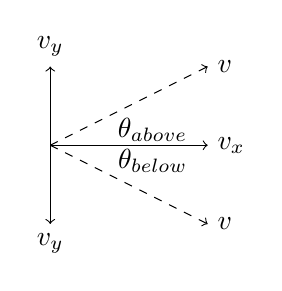
\begin{tikzpicture}
		\draw[->] (0, 0) -- (0, -1) node[below]{$v_y$};
		\draw[->] (0, 0) -- (0, 1) node[above]{$v_y$};
		\draw[->] (0, 0) -- (2, 0) node[right]{$v_x$};
		\draw[dashed, ->] (0, 0) -- (2, 1) node[right]{$v$};
		\draw[dashed, ->] (0, 0) -- (2, -1) node[right]{$v$};

		\node at (1.3, 0.2) {$\theta_{\text{above}}$};
		\node at (1.3, -0.2) {$\theta_{\text{below}}$};
	\end{tikzpicture}
\end{center}
From the above, we see that
$$ \tan\theta = \frac{v_x}{v_y} $$
into which, if we plug in the values of $v_x$ and $v_y$, we obtain an equation
in which $\theta$ can be solved for.

\subsection{Equilibrium of a rigid body}
\begin{point}
Calculate the moment of a force about a point
\end{point}
The \define{moment} of a force $F$, about a point $O$ is $F \times d$, where
$d$ is the perpendicular distance from the point $O$ to the line of action of
the force $F$. If the distance between the force and the point $O$ is zero,
there is no turning effect. The unit of moment is Newton metres: \SI{}{Nm}.
Thus,
$$ \boxed{\tau = Fd} $$

For a force applied at an angle $\theta$ from the perpendicular of the line 
drawn from the pivot to the force the moment comes out to be
$$ \boxed{\tau = Fd\cos\theta} $$
Here, we are simply finding the component of the force perpendicular to the
distance, $F\cos\theta$, and multiplying the distance $d$ to it.

In general, there are two types of moments about a pivot: clockwise and
anticlockwise moment. If the totals of the two moments about a pivot comes out
to be equal, the object is said to be in \emph{rotatonal} 
\define{equilibrium}. If the clockwise moment is greater, the object turns
clockwise and same for if the anticlockwise moment is greater.
\begin{point}
Use the result that the effect of gravity on a rigid
body is equivalent to a single force acting at
the centre of mass of the body, and identify the
position of the centre of mass of a uniform body
using considerations of symmetry
\end{point}
Consider a rod of length \SI{2}{m} and mass \SI{5}{kg}. We add a mass of 
\SI{3}{kg} to one end. This rod hangs from a point $O$, which is the end
opposite to where the mass is added. Thus the total moment, which is clockwise
for this rod is
\begin{align*}
	\tau &= (1)(5g) + (2)(3g) \\
		 &= 11g
\end{align*}
If we now consider the force coming from a point whose distance from $O$ is
$\bar{x}$
\begin{align*}
	\tau &= 11g \\
	\implies (5g + 3g)(\bar{x}) &= 11g \\
	\implies \bar{x} &= \frac{11}{8}
\end{align*}
Thus, the total moment of the rod may be said to be that of one force, 
\SI{8}{N}  at a distance of $11/8~\si{\metre}$ from $O$.

Consider a two-dimensional case such as a framework with masses added. This
gives us coordinates for the centre of mass.
